\begin{SCfigure}
  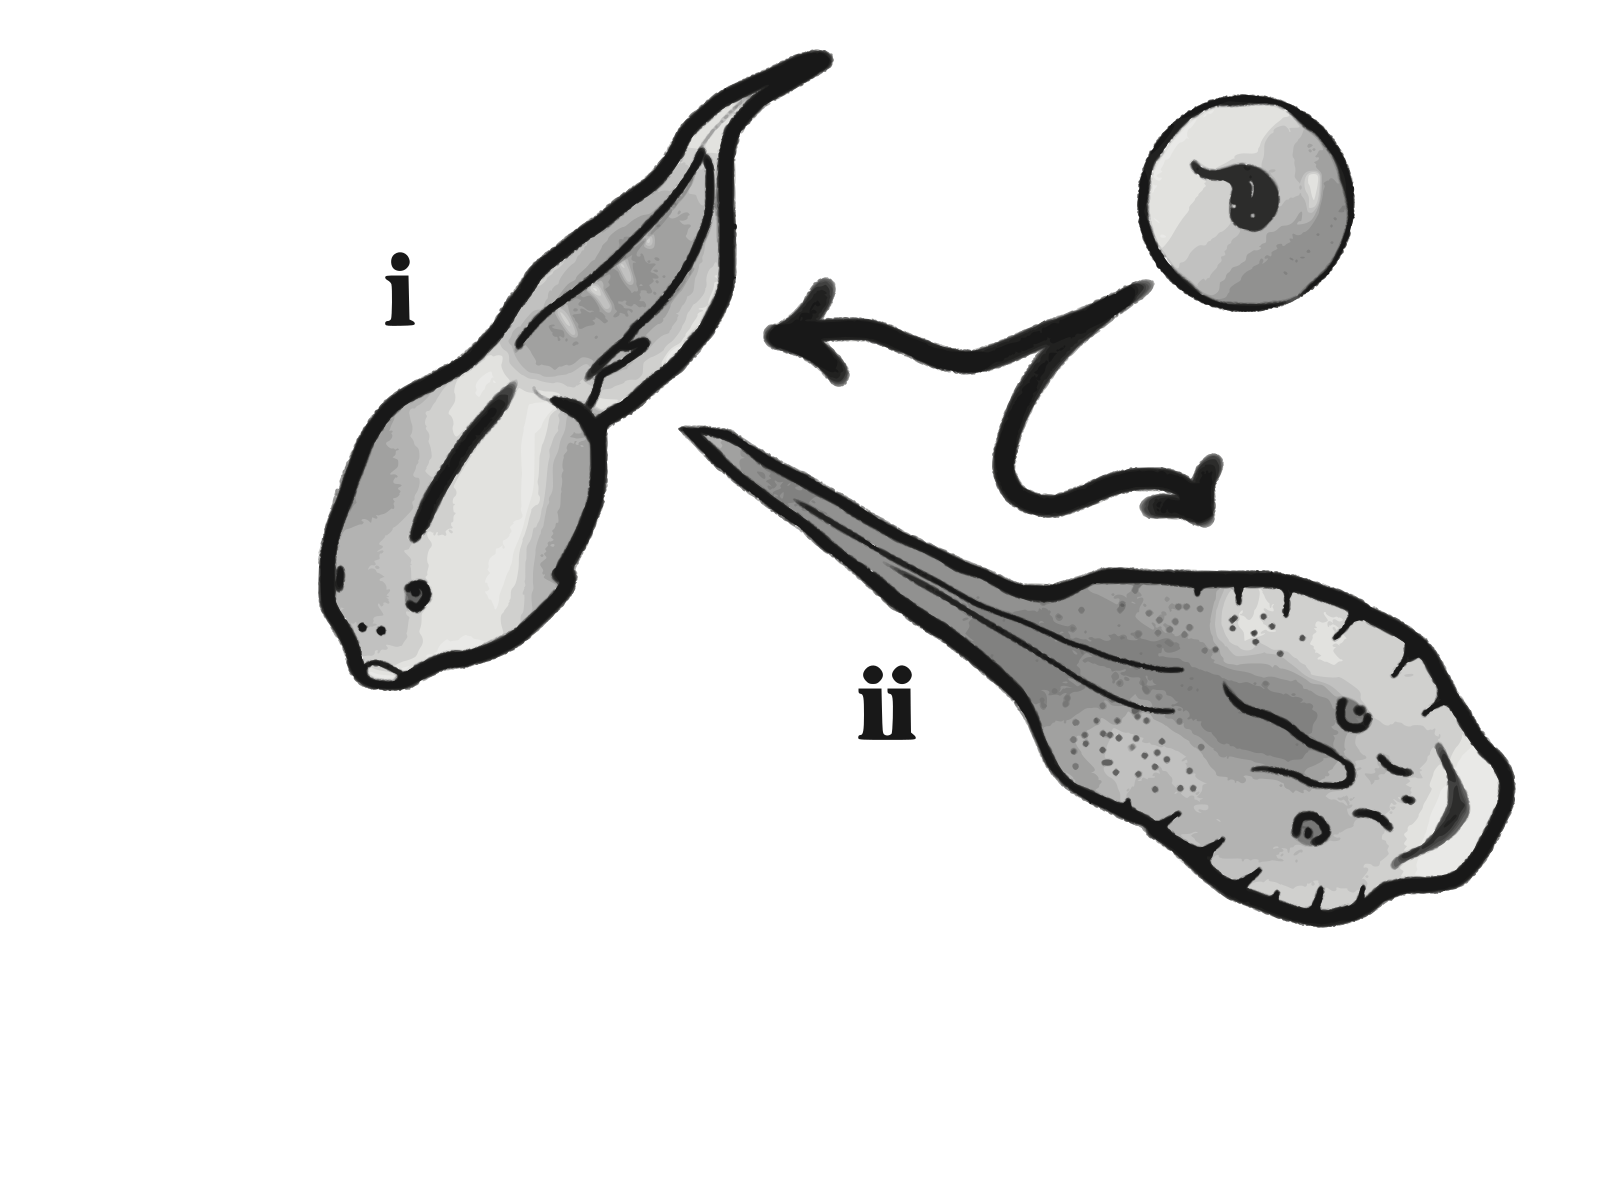
\includegraphics[width=0.5\textwidth]{img/tadpoles}
  %\captionsetup{singlelinecheck=off,justification=raggedright}
  \caption[Illustration of Indirect Plasticity in \textit{Spea multiplicata}]{An illustration of the alternate phenotypic forms of \textit{Spea multiplicata}. Form $i$ is known as the omnivorous form while form $ii$ is known as the carnivorous form. Developing tadpoles assume one or another of these forms on the basis of environmental signaling, thought to be the consumption of brine shrimp \cite{Pfennig1992PolyphenismStrategy}.}
  \label{fig:spea_multiplicata}
\end{SCfigure}
